% -----------------------------------------------------------------------
% Dokumentation der Vorlage f�r Texte
% -----------------------------------------------------------------------
\documentclass[enabledeprecatedfontcommands, fontsize=12pt,
     open=right, a4paper,
     twoside, DIV=11,
     abstractoff,
     headsepline,
     numbers=noenddot,
     BCOR=15mm,
     headings=standardclasses,
     headings=big]{scrbook}
\KOMAoptions{cleardoublepage=empty}
%
% Header f�r Variablen  wie Vorlesung, Semester, Pfade zu Aufgaben, Bildern, ...
% Variablen f�r das Semester, die Vorlesung ...
\newcommand{\theSemester}{Wintersemester~2021/22}
% Variable f�r die Vorlesung
\newcommand{\theClass}{Styles and More}
% Variable f�r den Studiengang
\newcommand{\theCourse}{Dokumentation der Datei setup.tex}
% Variable f�r den Hochschul-Namen
\newcommand{\theSchool}{Hochschule~Kaiserslautern}
% Variable f�r den Dozenten
\newcommand{\theTeacher}{Manfred~Brill}

%
% Verzeichnisse f�r �bungsaufgaben, Bitmaps, ...
%

% Verzeichnis f�r die �bungsaufgaben und Musterl�sungen
\newcommand{\exercisePath}{./Uebungsaufgaben/}
% Verzeichnis f�r  Bilder
\newcommand{\imagePath}{./images}

%
% Abbildungen f�r die Titelseite oder spezielle Markierungen
%
% Default-Titelbild der Lehrveranstaltung
\newcommand{\titleImage}{\imagePath/tugboat}
% Abbildung f�r die Angabe von Begleittexten
\newcommand{\lesenImage}{\imagePath/Misc/buchicon}
% Abbildung f�r die Angabe von vertiefenden Texten
\newcommand{\vertiefenImage}{\imagePath/Misc/reading}
% Abbildung f�r eine Marginalie zum Praxisbezug
\newcommand{\praxisImage}{\imagePath/Misc/gabel}
% Einstellungen
% ---------------------------------------------------------------------
% Vorlage f�r Dokumente, die auf report oder book basieren
% Voraussetzung: spezifische Variable wie \imagePath
% oder \theSemester sind bereits definiert.
% ---------------------------------------------------------------------
\typeout{Einstellung f�r Texte auf report/book-Basis}
\typeout{     (C) Manfred Brill}
\typeout{     Version 1.5 Oktober 2020}
\typeout{     PDF-Support f�r LaTeX-Grafiken}
\typeout{     Bei Verwendung von dvi -> ps -> pdf mb.sty verwenden!}
\usepackage{mbPDF}
\usepackage{mbmath}
\usepackage{textcomp}
% Array-Paket f�r mehr Kontrolle der Tabellen
\usepackage{array}
% ifthen f�r Ein- und Ausblenden der L�sungen.
\usepackage{ifthen}
% Paket f�r Postscript Pi-Fonts
\usepackage{pifont}
% Mit Hilfe des Package caption stellen wir sicher, dass \ref im PDF-Reader nicht
% zur Beschriftung, sondern zur Abbildung springt.
\usepackage{caption}
% Paket f�r das einfache Umdefinieren von Listen
\usepackage[shortlabels]{enumitem}
% Alphabetischer Index
\usepackage{imakeidx}
\makeindex[title=Index,columns=2,options=-s myGerman, intoc=true]
% Kopf- und Fusszeilen mit KoMaScript
\usepackage[automark, headsepline]{scrlayer-scrpage}
% Darstellen von Hierarchien wie eine Unity-Szene:
\usepackage{dirtree}
%
\pagestyle{scrheadings}
\clearscrheadfoot
% Kopfzeile definieren
\ihead{\headmark}
\ohead[]{\pagemark}
\chead{}
\pagestyle{scrheadings}
% Zentral definierte Variablen
% Abk�rzungen, Namen, ...
% -------------------------------------------------------------------
% variablen.tex
% Variablen f�r Werkzeuge, Begriffe, Firmen
% Stand: Juni 2017
% Liegt zentral in texmf-local/tex/latex/MB
% -------------------------------------------------------------------
% Programmiersprachen
\newcommand{\java}{\texttt{Java}}
\newcommand{\cpp}{\texttt{C++}}
\newcommand{\cl}{\texttt{C}}
\newcommand{\csharp}{\texttt{C\#}}
\newcommand{\php}{\texttt{PHP}}
\newcommand{\py}{\texttt{Python}}
\newcommand{\perl}{\texttt{Perl}}
\newcommand{\fc}{\texttt{Fortran}}
\newcommand{\obc}{\texttt{Objective C}}
\newcommand{\js}{\texttt{JavaScript}}
\newcommand{\omp}{\texttt{OpenMP}}
\newcommand{\mpi}{\texttt{MPI}}
\newcommand{\ocl}{\texttt{OpenCL}}
\newcommand{\cuda}{\texttt{CUDA}}
% Datei-Formate
\newcommand{\html}{\texttt{HTML}}
\newcommand{\xml}{\texttt{XML}}
\newcommand{\json}{\texttt{JSON}}
\newcommand{\rtf}{\texttt{RTF}}
\newcommand{\pdf}{\texttt{PDF}}
%
\newcommand{\sccs}{\texttt{SCCS}}
\newcommand{\rcs}{\texttt{RCS}}
\newcommand{\cvs}{\texttt{CVS}}
\newcommand{\svn}{\texttt{SVN}}
\newcommand{\subversion}{\texttt{Subversion}}
\newcommand{\git}{\texttt{Git}}
\newcommand{\github}{\texttt{GitHub}}
\newcommand{\githubDesktop}{\texttt{GitHub Desktop}}
\newcommand{\gitkraken}{\texttt{GitKraken}}
\newcommand{\gittortoise}{\texttt{TortoiseGit}}
\newcommand{\gittree}{\texttt{Sourcetree}}
\newcommand{\bitbucket}{\texttt{BitBucket}}
\newcommand{\mercurial}{\texttt{Mercurial}}
\newcommand{\pf}{\texttt{Perforce}}
\newcommand{\pfv}{\texttt{P4V}}
\newcommand{\pfc}{\texttt{p4}}
\newcommand{\pfmerge}{\texttt{P4Merge}}
\newcommand{\pfsand}{\texttt{P4.Sandbox}}

\newcommand{\vi}{\texttt{vi}}
\newcommand{\emacs}{\texttt{Emacs}}
%
\newcommand{\javadoc}{\texttt{Javadoc}}
\newcommand{\xmldoc}{\texttt{XMLdoc}}
\newcommand{\sandcastle}{\texttt{Sandcastle}}
\newcommand{\doxy}{\texttt{Doxygen}}
\newcommand{\doxyVersion}{\texttt{$1.8.7$}}
\newcommand{\doxywizard}{\texttt{Doxywizard}}
\newcommand{\graphviz}{\texttt{Graphviz}}
%
\newcommand{\logj}{\texttt{Log4j}}
\newcommand{\slfj}{\texttt{SLF4J}}
\newcommand{\logback}{\texttt{LOGBack}}
\newcommand{\jul}{\texttt{Java Logging API}}
\newcommand{\commonsLog}{\texttt{Apache Commons LoggingJ}}
\newcommand{\boostlog}{\texttt{Boost.Log}}
\newcommand{\glog}{\texttt{Google Logging Library}}
%
\newcommand{\junit}{\texttt{JUnit}}
\newcommand{\xunit}{\texttt{xUnit}}
\newcommand{\nunit}{\texttt{NUnit}}
\newcommand{\xunitnet}{\texttt{xUnit.net}}
\newcommand{\ctest}{\texttt{CTest}}
%
\newcommand{\ssh}{\texttt{ssh}}
\newcommand{\sftp}{\texttt{sftp}}
\newcommand{\make}{\texttt{make}}
\newcommand{\ant}{\texttt{Ant}}
\newcommand{\maven}{\texttt{Maven}}
\newcommand{\gradle}{\texttt{Gradle}}
\newcommand{\msbuild}{\texttt{MSBuild}}
\newcommand{\mstest}{\texttt{MSTest}}
\newcommand{\cmake}{\texttt{CMake}}
\newcommand{\jenkins}{\texttt{Jenkins}}
\newcommand{\ccontrol}{\texttt{cruisecontrol}}
\newcommand{\cdash}{\texttt{CDash}}
%
\newcommand{\eclipse}{\texttt{Eclipse}}
\newcommand{\vs}{\texttt{Visual Studio}}
\newcommand{\mono}{\texttt{Mono}}
\newcommand{\monodev}{\texttt{MonoDevelop}}
%
\newcommand{\openO}{\texttt{OpenOffice}}
\newcommand{\Qt}{\texttt{Qt}}
\newcommand{\firefox}{\texttt{Mozilla Firefox}}
\newcommand{\kde}{\texttt{KDE}}
%
\newcommand{\ms}{\texttt{Microsoft}}
\newcommand{\net}{\texttt{.NET}}
\newcommand{\sun}{\texttt{SUN}}
\newcommand{\ora}{\texttt{Oracle}}
\newcommand{\apache}{\texttt{Apache}}
\newcommand{\windows}{\texttt{Windows}}
\newcommand{\cyg}{\texttt{Cygwin}}
\newcommand{\linux}{\texttt{Linux}}
\newcommand{\unix}{\texttt{Unix}}
\newcommand{\osx}{\texttt{MacOS X}}
\newcommand{\android}{\texttt{Android}}
% VR Software
\newcommand{\unity}{\texttt{Unity}}
\newcommand{\verUnity}{\texttt{$2018.2$}}
\newcommand{\unreal}{\texttt{Unreal}}
\newcommand{\verUnreal}{\texttt{4}}
\newcommand{\juggler}{\texttt{VRJuggler}}
\newcommand{\cavelib}{\texttt{CAVELib}}
\newcommand{\gadgeteer}{\texttt{Gadgeteer}}
\newcommand{\vrpn}{\texttt{VRPN}}
\newcommand{\mvr}{\texttt{MiddleVR}}
\newcommand{\verMvr}{\texttt{$1.7.0.7$}}
% Computergrafik und Werkzeuge
\newcommand{\direct}{\texttt{Direct3D}}
\newcommand{\gl}{\texttt{OpenGL}}
\newcommand{\para}{\texttt{ParaView}}
\newcommand{\vtk}{\texttt{VTK}}
% R und anderes zur Datenanalyse
% \R ist schon definiert (Mathematik!)
\newcommand{\Rsoft}{\texttt{R}}
\newcommand{\Rstudio}{\texttt{RStudio}}
\newcommand{\verR}{\texttt{$3.3.3$}}
\newcommand{\mondrian}{\texttt{Mondrian}}
\newcommand{\tableau}{\texttt{Tableau}}
% LaTeX
\newcommand{\jabref}{\texttt{JabRef}}
\newcommand{\bibtex}{\textsc{Bib}\negthinspace\TeX}

% Farben
% ---------------------------------------------------------------------------------------
% Farben, f�r Folien und andere Dinge.
% Version vom Juli 2015 mit neuer Fachbereichsfarbe
%
% Letzte �nderung: 1.9.2015
%
% Um diese Datei zu verwenden muss Sie in texmf-local/MB kopiert werden
% und TeX muss aktualisiert werden!
% ---------------------------------------------------------------------------------------
\definecolor{light}{gray}{.75}
\definecolor{LightGray}{rgb}{0.24,0.24,0.24}
%   Farben rot gr�n blau f�r Koordinatenachsen
\definecolor{wred}{rgb}{0.8, 0.0, 0.0}
\definecolor{wgreen}{rgb}{0.0, 0.8, 0.0}
\definecolor{wblue}{rgb}{0.0, 0.0, 0.8}
\definecolor{wyellow}{rgb}{1.0, 1.0, 0.0}
\definecolor{wcyan}{rgb}{0.0, 1.0, 1.0}
% Fachbereichsfarbe neu
\definecolor{colorDepartment}{rgb}{0.16, 0.71, 0.86}
% Listings
\definecolor{lstback}{gray}{0.85}
%

%
\raggedbottom
\setlength{\parskip}{2.0ex}
\setlength{\parindent}{0.0cm}
% Verhindert Schusterjungen und Hurenkinder
\clubpenalty = 10000
\widowpenalty = 10000
\displaywidowpenalty = 10000
%
\setcounter{secnumdepth}{2}
\setcounter{tocdepth}{2}
% Abst�nde zwischen Caption und Bild/Tabelle
\setlength\abovecaptionskip          {0.4em}
\setlength\belowcaptionskip          {0.2em}
% Anteil der Grafiken auf einer Seite sehr hoch setzen
% Damit wird verhindert, dass bei vielen Abbildungen im Text die
% Abbildungen ans Ende des PDF geschoben werden.
\renewcommand{\topfraction}{0.99}
\renewcommand{\textfraction}{0.0001}
% Literatur-Stil
\bibliographystyle{geralpha}
% Font und Fettdruck f�r Tabelle/Abbildung (neu, jetzt mit komascript!
% MB, 28/07/2017
\addtokomafont{caption}{\small}
\setkomafont{captionlabel}{\bfseries}
% Einstellung f�r Gliederungs�berschriften mit KoMaScript
\RedeclareSectionCommands[
  beforeskip=-.5\baselineskip,
  afterskip=.25\baselineskip
]{section,subsection,subsubsection}
%
% listings-Paket f�r Quelltexte
%++++++++++++++++++++++++++++++++++++++++++++++++++++++++++++++++
%   Hintergrundfarbe von Quellcode
\definecolor{lstback}{gray}{0.85}
\lstloadlanguages{Java}
\lstset{language=Python}
\lstset{backgroundcolor=\color{lstback}}
\lstset{extendedchars=true}
\lstset{showstringspaces = false}
\lstset{keywordstyle=\bfseries} % Keywords fett
\lstset{basicstyle = \ttfamily \small}
\lstset{breaklines=true, breakatwhitespace=true} % Zeilenumbruch in listings
% Kommando f�r den Flattersatz bei nebeneinander liegenden Abbildungen
\newcommand*{\flatter}{\setlength{\rightskip}{0pt plus 2cm}}
% Anteil der Grafiken h�her auf jeder Seite!
\renewcommand{\textfraction}{0.001}
%
% Schritte in einer Aufz�hlung, daf�r einen Z�hler (schritt) und die Umgebung
% schritte definieren.
\newcounter{schritt}
\newenvironment{schritte}%
{\begin{list}%
{Schritt \arabic{schritt}:}%
{\usecounter{schritt}\settowidth{\labelwidth}{Schritt 1:}%
\setlength{\leftmargin}{\labelwidth}\addtolength\leftmargin{\labelsep}%
\parsep0.0ex\partopsep-0.3ex\itemsep2pt\topsep0.0ex}}{\end{list}}
%   Taste
\newcommand*{\taste}[1]{\small\textsf{#1}\normalsize}
%   gesch�tzte Namen (NICHT in chapter, section usw. verwenden!)
\newcommand*{\name}[1]{\textsl{#1}}
%   Fachbegriffe/Erkl�rung von Abk�rzungen
\newcommand*{\begriff}[1]{\index{#1}\textit{#1}}
%
\newcommand{\algorithmus}[2]{%
\vspace{4pt}\fboxsep 1mm \framebox[140mm]
{\parbox{135mm}{{\textbf{#1}}\vspace{2pt}#2}}\vspace{4pt}}
%
%   Dateinamen/Pfade
\newcommand*{\datei}[1]{\texttt{#1}\normalsize}
%   Tip (in einer Box)
\newcommand{\tip}[1]{%
\vspace{4pt}\fboxsep 1mm \framebox[140mm]
{\parbox{135mm}{{\textbf{Tipp}}:\\ #1}}\vspace{4pt}}
%
%   Reflektion (in einer Box)
\newcommand{\reflection}[1]{
\begin{quote}\fboxsep 3mm\framebox[140mm][c]{\parbox{130mm}{{\textbf Reflektion:\\}#1}}\end{quote}}
%
% Angabe im Begleittext, was die Studierenden lesen sollen (in einer Box)
\newcommand{\lesen}[1]{%
\begin{minipage}[c]{2.5cm}
\includegraphics[width=0.8\textwidth]{\lesenImage}%
\end{minipage}%
\begin{minipage}[t]{12cm}%
#1%
\end{minipage}}
%
%
%   Angabe im Begleittext, was die Studierenden lesen sollen (in einer Box)
%   Dieses Icon wird f�r Angaben verwendet, die nicht verpflichtend zu lesen
%   sind. Also "nice-to-have", "wenn sie noch Zeit haben".
%   Im Gegensatz zu lesen, was einen verpflichtenden Charakter hat.
\newcommand{\vertiefen}[1]{%
\begin{minipage}[b]{2.5cm}
\includegraphics[width=0.8\textwidth]{\vertiefenImage}%
\end{minipage}%
\begin{minipage}[b]{12cm}%
#1%
\end{minipage}}
%
% Ein Counter f�r die Kontrollfragen. Wir z�hlen diesen Counter selbst hoch
% mit einem entsprechenden Kommando, das wir in \item verwenden.
\newcounter{kontrollCounter}[chapter]
\newcommand{\kontroll}[0]{
    \refstepcounter{kontrollCounter}
    % Kapitelnummer.Z�hler f�r das Item
    \arabic{chapter}.\arabic{kontrollCounter}
    % Das Label ist bis auf weiteres "kontrolle:Kapitelnummer:kontrollcounter
    \label{kontrolle:\arabic{chapter}:\arabic{kontrollCounter}}
}
% Definition der Kontrollfrage; die Nummerierung
% f�r das ganze erhalten wir mit Hilfe von \item{\kontroll}.
\newcommand{\kontrollfrage}[1]{%
\begin{minipage}[c]{1.85cm}
\huge{\ding{46}}%
\end{minipage}%
\begin{minipage}[t]{12cm}%
\begin{itemize}#1%
\end{itemize}%
\end{minipage}}
% Schalter f�r das ein- und ausblenden der Musterl�sungen
\newboolean{solutions}
%
% Dateinamen
\newcommand{\filename}[1]{%
\ifthenelse{\boolean{solutions}}{\framebox[50mm]{\parbox{40mm}{\textbf #1}}\vspace{6pt}}{}}
%
% Theorem-Umgebung f�r die �bungsaufgaben
% Wichtig: alle Attribute einstellen, dann die neue
% theorem-Umgebung mit newtheorem definieren!
% Oder, wie hier, durch das Einschlie�en in {}
%
{
% Zeilenumbruch bei Aufgaben-�berschrift
\theoremstyle{break}
% "Normaler" Font im Text
\theorembodyfont{\normalfont}
% Kapitelweise neu nummerieren
\newtheorem{auftitle}{Aufgabe}[chapter]
}
%
% Definition f�r die Kennzeichnung der �bungsaufgaben
%
\newcommand{\uebung}{%
\vspace*{11pt}%
\begin{tabular}{@{}p{2.25cm}@{}p{11.7cm}}%
\huge{\ding{45}}&\Large{\textbf{�bungsaufgaben}}%
\end{tabular}%
}
% Ein Counter f�r die �bungsaufgaben. Wir z�hlen diesen Counter selbst hoch
% mit einem entsprechenden Kommando, das wir in \item verwenden.
\newcounter{aufgabenCounter}[chapter]
\newcommand{\auf}[0]{
    \refstepcounter{aufgabenCounter}
    % Kapitelnummer.Z�hler f�r das Item
    \arabic{chapter}.\arabic{aufgabenCounter}
}
% Der Text der Aufgaben steht im Ordner ../Uebungsaufgaben/aufgaben/aufgabenstellungen.
% Die Struktur ist so wie in den Mathematikvorlesungen.

% Umgebungen f�r Satz, Definition, Beweis, ... . Wir orientieren uns am Mathematik-Buch,
% dort gab es diese Umgebungen auch schon. Im Grunde sind das einfach
% wieder theorem-Umgebungen.
{
\setlength\theorempreskipamount{5pt plus 3pt minus 1.5pt}
\setlength\theorempostskipamount{5pt plus 1pt minus 1pt}
% "Normaler" Font im Text
\theorembodyfont{\normalfont}
% Die Namen sind so gew�hlt, dass sie kompatibel zu Beamer sind; dann k�nnen
% wir den Text aus Folien kopieren und umgekehrt auch.
\newtheorem{Satz}{Satz}[chapter]
\newtheorem{Beweis}{Beweis}[chapter]
\newtheorem{Fakt}{Fakt}[chapter]
\newtheorem{Definition}{Definition}[chapter]
}
% Text mit Pfad, der vorher im Dokument definiert ist.
\newcommand{\aufgabentext}[1]{\renewcommand{\labelenumi}{\alph{enumi})}\auftitle\label{#1}\input{\exercisePath/aufgaben/aufgabenstellungen/#1}}
% Funktion f�r die L�sungs-Hinweise f�r eine Aufgabe. Der Text
% steht analog zu den �bungsaufgaben im Ordner aufgaben/loesungen.
\newcommand{\hinweistext}[1]{\renewcommand{\labelenumi}{\alph{enumi})}\input{\exercisePath/aufgaben/loesungen/#1}}
% Und jetzt die Funktionen, die wir im Text aufrufen
\newcommand{\aufgabe}[1]{\aufgabentext{#1}}
% L�sungshinweise im Anhang
\newcommand{\hinweis}[1]{\subsubsection*{Aufgabe \ref{#1}} \hinweistext{#1}}
%
% Marginalien
%
\newcommand{\randnotiz}[1]{\marginpar{\small{\textbf{#1}}}}
%
% Gabelschl�ssel als Marginalie und Hinweis auf Praxisbezug
\newcommand{\praxisbezug}[0]{\randnotiz{\includegraphics[width=1cm]{\praxisImage}}}
%
% alert aus beamer-Folien zu emph machen
\newcommand*{\alert}[1]{\emph{#1}}
%
% Das Argument ist der Titel des Dokuments.
%
\newcommand{\titelseite}[1]{%
% Titelseite
\pagenumbering{roman}%
\thispagestyle{empty}%
\begin{titlepage}%
% Volle Zeilenbreite verwenden!
\centering%
\vspace*{0.5cm}%

\Huge{\textbf{\theClass{}}}\\\vspace*{0.5cm}%

\Huge{\textbf{#1}}%

\vspace*{1.0cm}%
\Large{\theSchool{}}%

\Large{\theTeacher{}}%

\Large{\theSemester{}}%
\end{titlepage}}
%
% Das obligatorische Argument ist der Titel des Dokuments.
% Als Default wird software-project.eps als Titelbild
% verwendet. Mit Hilfe eines optionalen Arguments kann
% ein anderes Bild verwendet werden!
% Beispiel: \titelseite[\imagePath/Misc/ameise]{Das Liebesleben der Ameisen}
%
\newcommand{\titelseiteMitBild}[2][\titleImage]{%
% Titelseite
\pagenumbering{roman}%
\thispagestyle{empty}%
\begin{titlepage}%
% Volle Zeilenbreite verwenden!
\centering%
\vspace*{0.5cm}%

\Huge{\textbf{\theClass{}}}\\\vspace*{0.5cm}%

\Huge{\textbf{#2}}%

\vspace*{3.0cm}%
\includegraphics[height=5cm]{#1}%

\vspace*{3.0cm}%
\Large{\theSchool{}}%

\Large{\theTeacher{}}%
\end{titlepage}}

% Darstellung von Punkten mit xpicture mit Hilfe von \pointmark
\renewcommand{\pointmark}{$\bullet$}
% Funktion, der die Koordinaten �bergeben werden und einen Punkt ausgibt
\newcommand{\drawPoint}[2]{\Put[c](#1, #2){\pointmark}}

% Testen: hier muss auch eine Definition f�r die Datens�tze hin,
% Datensatz-Texte und Daten in eigener Datei
\newcommand{\dataset}[2]{\textbf{\large Datensatz #1}\vspace*{0.3cm}\hrule\label{#2}\input{\exercisePath/datasets/#2}} 
%
% Hyperref-Optionen f�r PDF-Files
% Dieses Paket muss als letztes eingebunden werden. Deshalb
% wird es hier "lokal" und nicht in setup.tex aufgef�hrt!
\usepackage[breaklinks]{hyperref}
\usepackage{breakurl}

\hypersetup{
pdftitle = {Vorlage f�r Lehrtexte an der Hochschule Kaiserslautern},
pdfauthor = {Manfred Brill},
pdfsubject = {Studienbrief, Vorlage, LaTeX, Fachbereich Informatik und Mikrosystemtechnik},
pdfkeywords = {Fachbereich Informatik und Mikrosystemtechnik, Hochschule Kaiserslautern},
pdfdisplaydoctitle = true,
pdfpagemode = UseThumbs,
colorlinks = false,
linkcolor = green,
linkbordercolor = {0 1 0},
pdfpagelayout = {SinglePage}
}

\urlstyle{same}

%
% Schalter f�r das Ein- und Ausblenden der L�sungen
\setboolean{solutions}{true}
%
% Beginn Dokument
%
\begin{document}
% Es gibt eine Titelseite mit und ohne Bild. Beide Varianten kann man hier testen,
% durch Verschieben des Kommentarzeichens.
%\titelseite{\LaTeX{}-Texte an der Hochschule Kaiserslautern}
\titelseiteMitBild[\imagePath/tugboat]{\LaTeX{}-Texte an der Hochschule Kaiserslautern}
%
% Inhaltsverzeichnis
%
\tableofcontents
\clearevenpage
\pagenumbering{arabic}
%
%
%
\chapter{Einleitung}
Dieses Dokument ist eine kurze Einf�hrung in eine Vorlage, die f�r Lehrbriefe in den Modulen
\emph{Stochastik f�r Informatiker}, \emph{Software Management Grundlagen},
\emph{Software Qualit�tsmanagement} und \emph{Datenanalyse mit R} erstellt wurde. Grundlage der Vorlage
waren Empfehlungen f�r die Formatierung von Lehrbriefen der ZFH f�r Microsoft Word (\cite{zfh_11}).

Das Dokument setzt voraus, dass Kenntnisse in \LaTeX{} vorhanden sind.
F�r das Literaturverzeichnis wird BibTeX eingesetzt.
Weitere Hinweise zu \LaTeX{} findet man in \cite{mittelbach_05} und \cite{kopka_02}.

Getestet wurden die Einstellungen auf Windows 10 mit MiKTeX 2.9 und auf Debian. Die Version aus dem Jahr 2015 wurde
 auch auf Fedora 17 mit TeXLive getestet.
%
%
%
\chapter{Pakete und Style Files}
\section{Aufbau der Hauptdatei}
Um den Header der Haupt-Datei nicht unn�tig lang zu machen wurden alle
Einstellungen in die Datei \datei{setup.tex}\index{setup.tex} verschoben. Dort werden die n�tigen Pakete geladen und alle weiteren Einstellungen durchgef�hrt.

Angaben zum Semester, zum Modul oder zum Dozenten sind in einer
vorher zu ladenden Datei definiert. In diesem vorliegenden Dokument wird die
Datei \datei{stammdaten.tex} verwendet. An dieser Stelle werden die Pfade
f�r die Bilder und die �bungsaufgaben definiert. Wenn man Abbildungen
f�r Randnotizen oder Lese-Anleitungen verwendet definiert man die
zu Bilder, die dazu einsetzt ebenfalls in dieser Datei.

Hier die Werte die f�r dieses Dokument verwendet wurden:
\begin{lstlisting}{}
% Variablen f�r das Semester, die Vorlesung ...
\newcommand{\theSemester}{Sommersemester~2019}
% Variable f�r die Vorlesung
\newcommand{\theClass}{Styles and More}
% Variable f�r den Studiengang
\newcommand{\theCourse}{Dokumentation der Datei setup.tex}
% Variable f�r den Hochschul-Namen
\newcommand{\theSchool}{Hochschule~Kaiserslautern}
% Variable f�r den Dozenten
\newcommand{\theTeacher}{Manfred~Brill}

% Verzeichnis f�r die �bungsaufgaben
\newcommand{\exercisePath}{../../Uebungsaufgaben/Stochastik}
% Verzeichnis f�r Bilder
\newcommand{\imagePath}{./images}

%
% Abbildungen f�r die Titelseite oder spezielle Markierungen
%
% Default-Titelbild der Lehrveranstaltung
\newcommand{\titleImage}{\imagePath/tugboat}
% Abbildung f�r die Angabe von Begleittexten
\newcommand{\lesenImage}{\imagePath/Misc/buchicon}
% Abbildung f�r die Angabe von vertiefenden Texten
\newcommand{\vertiefenImage}{\imagePath/Misc/reading}
% Abbildung f�r eine Marginalie zum Praxisbezug
\newcommand{\praxisImage}{\imagePath/Misc/gabel}
% Abbildung f�r ein Smiley
\newcommand{\smileImage}{\imagePath/Misc/smilie} 
\end{lstlisting}
Makros und Funktionen verwenden diese Variablen, so dass Namen, Semester und anderes einfach zu ver�ndern ist,
indem man diese Datei anpasst. Die hier dargestellten Werte
findet man unter anderem auf der Titelseite.

Weiter gibt es die Datei \datei{pdfsetup.tex}, in der Angaben f�r die PDF-Dateien
gemacht werden. Insbesondere wird mit \lstinline$\hypersetup$ eingestellt, dass Links
in gr�n im PDF dargestellt werden, und dass URLs im Text mit Zeilenumbruch dargestellt werden:
\begin{lstlisting}{}
\usepackage[breaklinks]{hyperref}
\usepackage{breakurl}

\hypersetup{
pdftitle = {Vorlage f�r Lehrtexte
an der Hochschule Kaiserslautern},
pdfauthor = {Manfred Brill},
pdfsubject = {Studienbrief, Vorlage, LaTeX,
Fachbereich Informatik und Mikrosystemtechnik},
pdfkeywords = {Fachbereich Informatik und Mikrosystemtechnik,
Hochschule Kaiserslautern},
pdfdisplaydoctitle = true,
pdfpagemode = UseThumbs,
colorlinks = false,
linkcolor = green,
linkbordercolor = {0 1 0},
pdfpagelayout = {SinglePage}
}

\urlstyle{same}
\end{lstlisting}
Vom Ergebnis kann man sich im Acrobat Reader �berzeugen, die Angaben in der Datei
werden in die Eigenschaften der PDF-Datei geschrieben.
Wichtig ist, dass die Funktion \lstinline$\hypersetup$ als letztes im Header durchgef�hrt wird.

Die Files f�r die Erstellung eines Studienbriefs oder �hnlicher Dokumente f�r die Lehre sind immer auf die gleiche Weise organisiert. Im Stamm-Verzeichnis befinden sich
\begin{itemize}
\item \datei{setup.tex},
\item \datei{pdfsetup.tex}.
\end{itemize}
Spezifische Variable werden in der Datei \datei{stammdaten.tex} definiert, die vor
\datei{setup.tex} ins Dokument eingef�gt wird.

Der Header dieses Dokuments lautet folgenderma�en:
\begin{lstlisting}{}
\documentclass[enabledeprecatedfontcommands, fontsize=12pt,
     open=right, a4paper,
     twoside, DIV=11,
     abstractoff,
     headsepline,
     numbers=noenddot,
     BCOR=15mm,
     headings=standardclasses,
     headings=big]{scrbook}
\KOMAoptions{cleardoublepage=empty}
% Header f�r Variablen wie Vorlesung, Semester,
% Pfade zu Aufgaben, Bildern, ...
% Variablen f�r das Semester, die Vorlesung ...
\newcommand{\theSemester}{Wintersemester~2021/22}
% Variable f�r die Vorlesung
\newcommand{\theClass}{Styles and More}
% Variable f�r den Studiengang
\newcommand{\theCourse}{Dokumentation der Datei setup.tex}
% Variable f�r den Hochschul-Namen
\newcommand{\theSchool}{Hochschule~Kaiserslautern}
% Variable f�r den Dozenten
\newcommand{\theTeacher}{Manfred~Brill}

%
% Verzeichnisse f�r �bungsaufgaben, Bitmaps, ...
%

% Verzeichnis f�r die �bungsaufgaben und Musterl�sungen
\newcommand{\exercisePath}{./Uebungsaufgaben/}
% Verzeichnis f�r  Bilder
\newcommand{\imagePath}{./images}

%
% Abbildungen f�r die Titelseite oder spezielle Markierungen
%
% Default-Titelbild der Lehrveranstaltung
\newcommand{\titleImage}{\imagePath/tugboat}
% Abbildung f�r die Angabe von Begleittexten
\newcommand{\lesenImage}{\imagePath/Misc/buchicon}
% Abbildung f�r die Angabe von vertiefenden Texten
\newcommand{\vertiefenImage}{\imagePath/Misc/reading}
% Abbildung f�r eine Marginalie zum Praxisbezug
\newcommand{\praxisImage}{\imagePath/Misc/gabel}
% Einstellungen
% ---------------------------------------------------------------------
% Vorlage f�r Dokumente, die auf report oder book basieren
% Voraussetzung: spezifische Variable wie \imagePath
% oder \theSemester sind bereits definiert.
% ---------------------------------------------------------------------
\typeout{Einstellung f�r Texte auf report/book-Basis}
\typeout{     (C) Manfred Brill}
\typeout{     Version 1.5 Oktober 2020}
\typeout{     PDF-Support f�r LaTeX-Grafiken}
\typeout{     Bei Verwendung von dvi -> ps -> pdf mb.sty verwenden!}
\usepackage{mbPDF}
\usepackage{mbmath}
\usepackage{textcomp}
% Array-Paket f�r mehr Kontrolle der Tabellen
\usepackage{array}
% ifthen f�r Ein- und Ausblenden der L�sungen.
\usepackage{ifthen}
% Paket f�r Postscript Pi-Fonts
\usepackage{pifont}
% Mit Hilfe des Package caption stellen wir sicher, dass \ref im PDF-Reader nicht
% zur Beschriftung, sondern zur Abbildung springt.
\usepackage{caption}
% Paket f�r das einfache Umdefinieren von Listen
\usepackage[shortlabels]{enumitem}
% Alphabetischer Index
\usepackage{imakeidx}
\makeindex[title=Index,columns=2,options=-s myGerman, intoc=true]
% Kopf- und Fusszeilen mit KoMaScript
\usepackage[automark, headsepline]{scrlayer-scrpage}
% Darstellen von Hierarchien wie eine Unity-Szene:
\usepackage{dirtree}
%
\pagestyle{scrheadings}
\clearscrheadfoot
% Kopfzeile definieren
\ihead{\headmark}
\ohead[]{\pagemark}
\chead{}
\pagestyle{scrheadings}
% Zentral definierte Variablen
% Abk�rzungen, Namen, ...
% -------------------------------------------------------------------
% variablen.tex
% Variablen f�r Werkzeuge, Begriffe, Firmen
% Stand: Juni 2017
% Liegt zentral in texmf-local/tex/latex/MB
% -------------------------------------------------------------------
% Programmiersprachen
\newcommand{\java}{\texttt{Java}}
\newcommand{\cpp}{\texttt{C++}}
\newcommand{\cl}{\texttt{C}}
\newcommand{\csharp}{\texttt{C\#}}
\newcommand{\php}{\texttt{PHP}}
\newcommand{\py}{\texttt{Python}}
\newcommand{\perl}{\texttt{Perl}}
\newcommand{\fc}{\texttt{Fortran}}
\newcommand{\obc}{\texttt{Objective C}}
\newcommand{\js}{\texttt{JavaScript}}
\newcommand{\omp}{\texttt{OpenMP}}
\newcommand{\mpi}{\texttt{MPI}}
\newcommand{\ocl}{\texttt{OpenCL}}
\newcommand{\cuda}{\texttt{CUDA}}
% Datei-Formate
\newcommand{\html}{\texttt{HTML}}
\newcommand{\xml}{\texttt{XML}}
\newcommand{\json}{\texttt{JSON}}
\newcommand{\rtf}{\texttt{RTF}}
\newcommand{\pdf}{\texttt{PDF}}
%
\newcommand{\sccs}{\texttt{SCCS}}
\newcommand{\rcs}{\texttt{RCS}}
\newcommand{\cvs}{\texttt{CVS}}
\newcommand{\svn}{\texttt{SVN}}
\newcommand{\subversion}{\texttt{Subversion}}
\newcommand{\git}{\texttt{Git}}
\newcommand{\github}{\texttt{GitHub}}
\newcommand{\githubDesktop}{\texttt{GitHub Desktop}}
\newcommand{\gitkraken}{\texttt{GitKraken}}
\newcommand{\gittortoise}{\texttt{TortoiseGit}}
\newcommand{\gittree}{\texttt{Sourcetree}}
\newcommand{\bitbucket}{\texttt{BitBucket}}
\newcommand{\mercurial}{\texttt{Mercurial}}
\newcommand{\pf}{\texttt{Perforce}}
\newcommand{\pfv}{\texttt{P4V}}
\newcommand{\pfc}{\texttt{p4}}
\newcommand{\pfmerge}{\texttt{P4Merge}}
\newcommand{\pfsand}{\texttt{P4.Sandbox}}

\newcommand{\vi}{\texttt{vi}}
\newcommand{\emacs}{\texttt{Emacs}}
%
\newcommand{\javadoc}{\texttt{Javadoc}}
\newcommand{\xmldoc}{\texttt{XMLdoc}}
\newcommand{\sandcastle}{\texttt{Sandcastle}}
\newcommand{\doxy}{\texttt{Doxygen}}
\newcommand{\doxyVersion}{\texttt{$1.8.7$}}
\newcommand{\doxywizard}{\texttt{Doxywizard}}
\newcommand{\graphviz}{\texttt{Graphviz}}
%
\newcommand{\logj}{\texttt{Log4j}}
\newcommand{\slfj}{\texttt{SLF4J}}
\newcommand{\logback}{\texttt{LOGBack}}
\newcommand{\jul}{\texttt{Java Logging API}}
\newcommand{\commonsLog}{\texttt{Apache Commons LoggingJ}}
\newcommand{\boostlog}{\texttt{Boost.Log}}
\newcommand{\glog}{\texttt{Google Logging Library}}
%
\newcommand{\junit}{\texttt{JUnit}}
\newcommand{\xunit}{\texttt{xUnit}}
\newcommand{\nunit}{\texttt{NUnit}}
\newcommand{\xunitnet}{\texttt{xUnit.net}}
\newcommand{\ctest}{\texttt{CTest}}
%
\newcommand{\ssh}{\texttt{ssh}}
\newcommand{\sftp}{\texttt{sftp}}
\newcommand{\make}{\texttt{make}}
\newcommand{\ant}{\texttt{Ant}}
\newcommand{\maven}{\texttt{Maven}}
\newcommand{\gradle}{\texttt{Gradle}}
\newcommand{\msbuild}{\texttt{MSBuild}}
\newcommand{\mstest}{\texttt{MSTest}}
\newcommand{\cmake}{\texttt{CMake}}
\newcommand{\jenkins}{\texttt{Jenkins}}
\newcommand{\ccontrol}{\texttt{cruisecontrol}}
\newcommand{\cdash}{\texttt{CDash}}
%
\newcommand{\eclipse}{\texttt{Eclipse}}
\newcommand{\vs}{\texttt{Visual Studio}}
\newcommand{\mono}{\texttt{Mono}}
\newcommand{\monodev}{\texttt{MonoDevelop}}
%
\newcommand{\openO}{\texttt{OpenOffice}}
\newcommand{\Qt}{\texttt{Qt}}
\newcommand{\firefox}{\texttt{Mozilla Firefox}}
\newcommand{\kde}{\texttt{KDE}}
%
\newcommand{\ms}{\texttt{Microsoft}}
\newcommand{\net}{\texttt{.NET}}
\newcommand{\sun}{\texttt{SUN}}
\newcommand{\ora}{\texttt{Oracle}}
\newcommand{\apache}{\texttt{Apache}}
\newcommand{\windows}{\texttt{Windows}}
\newcommand{\cyg}{\texttt{Cygwin}}
\newcommand{\linux}{\texttt{Linux}}
\newcommand{\unix}{\texttt{Unix}}
\newcommand{\osx}{\texttt{MacOS X}}
\newcommand{\android}{\texttt{Android}}
% VR Software
\newcommand{\unity}{\texttt{Unity}}
\newcommand{\verUnity}{\texttt{$2018.2$}}
\newcommand{\unreal}{\texttt{Unreal}}
\newcommand{\verUnreal}{\texttt{4}}
\newcommand{\juggler}{\texttt{VRJuggler}}
\newcommand{\cavelib}{\texttt{CAVELib}}
\newcommand{\gadgeteer}{\texttt{Gadgeteer}}
\newcommand{\vrpn}{\texttt{VRPN}}
\newcommand{\mvr}{\texttt{MiddleVR}}
\newcommand{\verMvr}{\texttt{$1.7.0.7$}}
% Computergrafik und Werkzeuge
\newcommand{\direct}{\texttt{Direct3D}}
\newcommand{\gl}{\texttt{OpenGL}}
\newcommand{\para}{\texttt{ParaView}}
\newcommand{\vtk}{\texttt{VTK}}
% R und anderes zur Datenanalyse
% \R ist schon definiert (Mathematik!)
\newcommand{\Rsoft}{\texttt{R}}
\newcommand{\Rstudio}{\texttt{RStudio}}
\newcommand{\verR}{\texttt{$3.3.3$}}
\newcommand{\mondrian}{\texttt{Mondrian}}
\newcommand{\tableau}{\texttt{Tableau}}
% LaTeX
\newcommand{\jabref}{\texttt{JabRef}}
\newcommand{\bibtex}{\textsc{Bib}\negthinspace\TeX}

% Farben
% ---------------------------------------------------------------------------------------
% Farben, f�r Folien und andere Dinge.
% Version vom Juli 2015 mit neuer Fachbereichsfarbe
%
% Letzte �nderung: 1.9.2015
%
% Um diese Datei zu verwenden muss Sie in texmf-local/MB kopiert werden
% und TeX muss aktualisiert werden!
% ---------------------------------------------------------------------------------------
\definecolor{light}{gray}{.75}
\definecolor{LightGray}{rgb}{0.24,0.24,0.24}
%   Farben rot gr�n blau f�r Koordinatenachsen
\definecolor{wred}{rgb}{0.8, 0.0, 0.0}
\definecolor{wgreen}{rgb}{0.0, 0.8, 0.0}
\definecolor{wblue}{rgb}{0.0, 0.0, 0.8}
\definecolor{wyellow}{rgb}{1.0, 1.0, 0.0}
\definecolor{wcyan}{rgb}{0.0, 1.0, 1.0}
% Fachbereichsfarbe neu
\definecolor{colorDepartment}{rgb}{0.16, 0.71, 0.86}
% Listings
\definecolor{lstback}{gray}{0.85}
%

%
\raggedbottom
\setlength{\parskip}{2.0ex}
\setlength{\parindent}{0.0cm}
% Verhindert Schusterjungen und Hurenkinder
\clubpenalty = 10000
\widowpenalty = 10000
\displaywidowpenalty = 10000
%
\setcounter{secnumdepth}{2}
\setcounter{tocdepth}{2}
% Abst�nde zwischen Caption und Bild/Tabelle
\setlength\abovecaptionskip          {0.4em}
\setlength\belowcaptionskip          {0.2em}
% Anteil der Grafiken auf einer Seite sehr hoch setzen
% Damit wird verhindert, dass bei vielen Abbildungen im Text die
% Abbildungen ans Ende des PDF geschoben werden.
\renewcommand{\topfraction}{0.99}
\renewcommand{\textfraction}{0.0001}
% Literatur-Stil
\bibliographystyle{geralpha}
% Font und Fettdruck f�r Tabelle/Abbildung (neu, jetzt mit komascript!
% MB, 28/07/2017
\addtokomafont{caption}{\small}
\setkomafont{captionlabel}{\bfseries}
% Einstellung f�r Gliederungs�berschriften mit KoMaScript
\RedeclareSectionCommands[
  beforeskip=-.5\baselineskip,
  afterskip=.25\baselineskip
]{section,subsection,subsubsection}
%
% listings-Paket f�r Quelltexte
%++++++++++++++++++++++++++++++++++++++++++++++++++++++++++++++++
%   Hintergrundfarbe von Quellcode
\definecolor{lstback}{gray}{0.85}
\lstloadlanguages{Java}
\lstset{language=Python}
\lstset{backgroundcolor=\color{lstback}}
\lstset{extendedchars=true}
\lstset{showstringspaces = false}
\lstset{keywordstyle=\bfseries} % Keywords fett
\lstset{basicstyle = \ttfamily \small}
\lstset{breaklines=true, breakatwhitespace=true} % Zeilenumbruch in listings
% Kommando f�r den Flattersatz bei nebeneinander liegenden Abbildungen
\newcommand*{\flatter}{\setlength{\rightskip}{0pt plus 2cm}}
% Anteil der Grafiken h�her auf jeder Seite!
\renewcommand{\textfraction}{0.001}
%
% Schritte in einer Aufz�hlung, daf�r einen Z�hler (schritt) und die Umgebung
% schritte definieren.
\newcounter{schritt}
\newenvironment{schritte}%
{\begin{list}%
{Schritt \arabic{schritt}:}%
{\usecounter{schritt}\settowidth{\labelwidth}{Schritt 1:}%
\setlength{\leftmargin}{\labelwidth}\addtolength\leftmargin{\labelsep}%
\parsep0.0ex\partopsep-0.3ex\itemsep2pt\topsep0.0ex}}{\end{list}}
%   Taste
\newcommand*{\taste}[1]{\small\textsf{#1}\normalsize}
%   gesch�tzte Namen (NICHT in chapter, section usw. verwenden!)
\newcommand*{\name}[1]{\textsl{#1}}
%   Fachbegriffe/Erkl�rung von Abk�rzungen
\newcommand*{\begriff}[1]{\index{#1}\textit{#1}}
%
\newcommand{\algorithmus}[2]{%
\vspace{4pt}\fboxsep 1mm \framebox[140mm]
{\parbox{135mm}{{\textbf{#1}}\vspace{2pt}#2}}\vspace{4pt}}
%
%   Dateinamen/Pfade
\newcommand*{\datei}[1]{\texttt{#1}\normalsize}
%   Tip (in einer Box)
\newcommand{\tip}[1]{%
\vspace{4pt}\fboxsep 1mm \framebox[140mm]
{\parbox{135mm}{{\textbf{Tipp}}:\\ #1}}\vspace{4pt}}
%
%   Reflektion (in einer Box)
\newcommand{\reflection}[1]{
\begin{quote}\fboxsep 3mm\framebox[140mm][c]{\parbox{130mm}{{\textbf Reflektion:\\}#1}}\end{quote}}
%
% Angabe im Begleittext, was die Studierenden lesen sollen (in einer Box)
\newcommand{\lesen}[1]{%
\begin{minipage}[c]{2.5cm}
\includegraphics[width=0.8\textwidth]{\lesenImage}%
\end{minipage}%
\begin{minipage}[t]{12cm}%
#1%
\end{minipage}}
%
%
%   Angabe im Begleittext, was die Studierenden lesen sollen (in einer Box)
%   Dieses Icon wird f�r Angaben verwendet, die nicht verpflichtend zu lesen
%   sind. Also "nice-to-have", "wenn sie noch Zeit haben".
%   Im Gegensatz zu lesen, was einen verpflichtenden Charakter hat.
\newcommand{\vertiefen}[1]{%
\begin{minipage}[b]{2.5cm}
\includegraphics[width=0.8\textwidth]{\vertiefenImage}%
\end{minipage}%
\begin{minipage}[b]{12cm}%
#1%
\end{minipage}}
%
% Ein Counter f�r die Kontrollfragen. Wir z�hlen diesen Counter selbst hoch
% mit einem entsprechenden Kommando, das wir in \item verwenden.
\newcounter{kontrollCounter}[chapter]
\newcommand{\kontroll}[0]{
    \refstepcounter{kontrollCounter}
    % Kapitelnummer.Z�hler f�r das Item
    \arabic{chapter}.\arabic{kontrollCounter}
    % Das Label ist bis auf weiteres "kontrolle:Kapitelnummer:kontrollcounter
    \label{kontrolle:\arabic{chapter}:\arabic{kontrollCounter}}
}
% Definition der Kontrollfrage; die Nummerierung
% f�r das ganze erhalten wir mit Hilfe von \item{\kontroll}.
\newcommand{\kontrollfrage}[1]{%
\begin{minipage}[c]{1.85cm}
\huge{\ding{46}}%
\end{minipage}%
\begin{minipage}[t]{12cm}%
\begin{itemize}#1%
\end{itemize}%
\end{minipage}}
% Schalter f�r das ein- und ausblenden der Musterl�sungen
\newboolean{solutions}
%
% Dateinamen
\newcommand{\filename}[1]{%
\ifthenelse{\boolean{solutions}}{\framebox[50mm]{\parbox{40mm}{\textbf #1}}\vspace{6pt}}{}}
%
% Theorem-Umgebung f�r die �bungsaufgaben
% Wichtig: alle Attribute einstellen, dann die neue
% theorem-Umgebung mit newtheorem definieren!
% Oder, wie hier, durch das Einschlie�en in {}
%
{
% Zeilenumbruch bei Aufgaben-�berschrift
\theoremstyle{break}
% "Normaler" Font im Text
\theorembodyfont{\normalfont}
% Kapitelweise neu nummerieren
\newtheorem{auftitle}{Aufgabe}[chapter]
}
%
% Definition f�r die Kennzeichnung der �bungsaufgaben
%
\newcommand{\uebung}{%
\vspace*{11pt}%
\begin{tabular}{@{}p{2.25cm}@{}p{11.7cm}}%
\huge{\ding{45}}&\Large{\textbf{�bungsaufgaben}}%
\end{tabular}%
}
% Ein Counter f�r die �bungsaufgaben. Wir z�hlen diesen Counter selbst hoch
% mit einem entsprechenden Kommando, das wir in \item verwenden.
\newcounter{aufgabenCounter}[chapter]
\newcommand{\auf}[0]{
    \refstepcounter{aufgabenCounter}
    % Kapitelnummer.Z�hler f�r das Item
    \arabic{chapter}.\arabic{aufgabenCounter}
}
% Der Text der Aufgaben steht im Ordner ../Uebungsaufgaben/aufgaben/aufgabenstellungen.
% Die Struktur ist so wie in den Mathematikvorlesungen.

% Umgebungen f�r Satz, Definition, Beweis, ... . Wir orientieren uns am Mathematik-Buch,
% dort gab es diese Umgebungen auch schon. Im Grunde sind das einfach
% wieder theorem-Umgebungen.
{
\setlength\theorempreskipamount{5pt plus 3pt minus 1.5pt}
\setlength\theorempostskipamount{5pt plus 1pt minus 1pt}
% "Normaler" Font im Text
\theorembodyfont{\normalfont}
% Die Namen sind so gew�hlt, dass sie kompatibel zu Beamer sind; dann k�nnen
% wir den Text aus Folien kopieren und umgekehrt auch.
\newtheorem{Satz}{Satz}[chapter]
\newtheorem{Beweis}{Beweis}[chapter]
\newtheorem{Fakt}{Fakt}[chapter]
\newtheorem{Definition}{Definition}[chapter]
}
% Text mit Pfad, der vorher im Dokument definiert ist.
\newcommand{\aufgabentext}[1]{\renewcommand{\labelenumi}{\alph{enumi})}\auftitle\label{#1}\input{\exercisePath/aufgaben/aufgabenstellungen/#1}}
% Funktion f�r die L�sungs-Hinweise f�r eine Aufgabe. Der Text
% steht analog zu den �bungsaufgaben im Ordner aufgaben/loesungen.
\newcommand{\hinweistext}[1]{\renewcommand{\labelenumi}{\alph{enumi})}\input{\exercisePath/aufgaben/loesungen/#1}}
% Und jetzt die Funktionen, die wir im Text aufrufen
\newcommand{\aufgabe}[1]{\aufgabentext{#1}}
% L�sungshinweise im Anhang
\newcommand{\hinweis}[1]{\subsubsection*{Aufgabe \ref{#1}} \hinweistext{#1}}
%
% Marginalien
%
\newcommand{\randnotiz}[1]{\marginpar{\small{\textbf{#1}}}}
%
% Gabelschl�ssel als Marginalie und Hinweis auf Praxisbezug
\newcommand{\praxisbezug}[0]{\randnotiz{\includegraphics[width=1cm]{\praxisImage}}}
%
% alert aus beamer-Folien zu emph machen
\newcommand*{\alert}[1]{\emph{#1}}
%
% Das Argument ist der Titel des Dokuments.
%
\newcommand{\titelseite}[1]{%
% Titelseite
\pagenumbering{roman}%
\thispagestyle{empty}%
\begin{titlepage}%
% Volle Zeilenbreite verwenden!
\centering%
\vspace*{0.5cm}%

\Huge{\textbf{\theClass{}}}\\\vspace*{0.5cm}%

\Huge{\textbf{#1}}%

\vspace*{1.0cm}%
\Large{\theSchool{}}%

\Large{\theTeacher{}}%

\Large{\theSemester{}}%
\end{titlepage}}
%
% Das obligatorische Argument ist der Titel des Dokuments.
% Als Default wird software-project.eps als Titelbild
% verwendet. Mit Hilfe eines optionalen Arguments kann
% ein anderes Bild verwendet werden!
% Beispiel: \titelseite[\imagePath/Misc/ameise]{Das Liebesleben der Ameisen}
%
\newcommand{\titelseiteMitBild}[2][\titleImage]{%
% Titelseite
\pagenumbering{roman}%
\thispagestyle{empty}%
\begin{titlepage}%
% Volle Zeilenbreite verwenden!
\centering%
\vspace*{0.5cm}%

\Huge{\textbf{\theClass{}}}\\\vspace*{0.5cm}%

\Huge{\textbf{#2}}%

\vspace*{3.0cm}%
\includegraphics[height=5cm]{#1}%

\vspace*{3.0cm}%
\Large{\theSchool{}}%

\Large{\theTeacher{}}%
\end{titlepage}}

% Darstellung von Punkten mit xpicture mit Hilfe von \pointmark
\renewcommand{\pointmark}{$\bullet$}
% Funktion, der die Koordinaten �bergeben werden und einen Punkt ausgibt
\newcommand{\drawPoint}[2]{\Put[c](#1, #2){\pointmark}}

% Spezifische Definitionen f�r die
Stochastik f�r Informatiker, Studiengang IT-Analyst
% Datensatz-Texte und Daten in eigener Datei
\newcommand{\dataset}[2]{\textbf{\large Datensatz #1}\vspace*{0.3cm}\hrule\label{#2}\input{\exercisePath/datasets/#2}} 
%
% Hyperref-Optionen f�r PDF-Files
% Dieses Paket muss als letztes eingebunden werden. Deshalb
% wird es hier "lokal" und nicht in setup.tex aufgef�hrt!
\usepackage[breaklinks]{hyperref}
\usepackage{breakurl}

\hypersetup{
pdftitle = {Vorlage f�r Lehrtexte an der Hochschule Kaiserslautern},
pdfauthor = {Manfred Brill},
pdfsubject = {Studienbrief, Vorlage, LaTeX, Fachbereich Informatik und Mikrosystemtechnik},
pdfkeywords = {Fachbereich Informatik und Mikrosystemtechnik, Hochschule Kaiserslautern},
pdfdisplaydoctitle = true,
pdfpagemode = UseThumbs,
colorlinks = false,
linkcolor = green,
linkbordercolor = {0 1 0},
pdfpagelayout = {SinglePage}
}

\urlstyle{same}

%
\end{lstlisting}
Solange wir noch \bibtex{} als Literaturverwaltung verwenden m�ssen
wir bei KoMaScript die Option \lstinline$enabledeprecatedfontcommands$ laden,
sonst kompilieren die \LaTeX{}-Texte nicht mehr.

Ein Blick auf den Satzspiegel zeigt, dass ein relativ gro�er Rand
gesetzt wird. Dies liegt daran, dass wir, wie wir noch sehen werden,
Marginalien, also Randnotizen, einsetzen. Wenn man darauf verzichtet
kann mit der dokumentierten Vorlage auch ein anderer Satzspiegel eingestellt werden!
%
\section{Die Datei setup.tex}
\subsection{Verwendete \LaTeX{}-Pakete}
Die Datei \datei{setup.tex} verwendet style files, die im Rahmen von B�chern
entstanden sind:
\datei{mbPDF.sty} und \datei{mbmath.sty}. Eine Dokumentation dazu
findet man in \cite{brill_18, brill_13b}. In \lstinline$mbPDF.sty$ werden die grundlegenden
Pakete geladen, Fonts und so weiter festgelegt. In \datei{mbmath.sty} gibt es auf der Basis
der AMS-Pakete weitere Definitionen f�r Funktionen und andere mathematischen
mathematischen Symbole. Werden diese nicht ben�tigt kann man diesen Eintrag l�schen.

Dar�ber hinaus werden die folgenden Pakete geladen:
\begin{itemize}
\item \lstinline$textcomp$
\item \lstinline$array$
\item \lstinline$ifthen$
\item \lstinline$pifont$
\item \lstinline$caption$
\item \lstinline$enumitem$ mit der Option \lstinline$shortlabels$
\item \lstinline$imakeidx$, mit
\begin{lstlisting}{}
\makeindex[title=Index,columns=2,options=-s german, intoc=true]
\end{lstlisting}
\item \lstinline$scrlayer-scrpage$ mit den Optionen
\lstinline$automark$ und \lstinline$headsepline$
\item \lstinline$hyperref$
\end{itemize}
In \lstinline$\makeindex$ wird der Index so eingestellt, dass er mit deutschen
Umlauten arbeiten kann und zweispaltig formatiert wird. Je nachdem wie der Index erstellt werden soll kann man dieses Paket weglassen und mit dem "`normalen"' Index arbeiten.

\tip{Wichtig ist, dass \lstinline$hyperref$ als \emph{letztes} Paket geladen wird.
Deshalb die Auslagerung f�r dieses Paket in die Datei \datei{pdfsetup.tex}.}
%
%
%
\subsection{Einstellungen und Funktionen}
Nach dem Laden der \LaTeX{}-Pakete werden noch einige Dateien geladen, die entweder
im aktuellen Verzeichnis oder zentral, in \datei{texmf-local}, liegen k�nnen.
Aktuell werden die folgenden Dateien geladen:
\begin{itemize}
\item \datei{variablen} f�r Begriffe wie Programmiersprachen, Software-Pakete, Versionen
und anderen Angaben,
\item \datei{colors} f�r Farben (z.b. die aktuelle Fachbereichsfarbe), und
\item \datei{coordinateSystems} f�r \LaTeX{}-Makros zum Zeichnen von Koordinatensystemen
mit \LaTeX{}-Vektorgrafik. Diese Datei ist als deprecated markiert und ist nur noch aus Kompatibilit�tsgr�nden enthalten.
\end{itemize}
Beispiele f�r Definitionen, die in diesen Dateien enthalten sind findet man weiter unten im Text.

Mit \lstinline$\raggedbottom$ wird eingestellt,
dass \LaTeX{} die Zeilen nicht auseinander zieht um eine Seite zu f�llen. Diese Einstellung
stammt aus der Zusammenarbeit mit dem Hanser-Verlag. Damit erh�lt man gleiche
Zeilenabst�nde. Verwendet man den \LaTeX{}-Default werden die Zeilen etwas verzogen,
um auf jede Seite den exakt gleichen Satzspiegel zu haben. Das m�gen Buchbinder
gar nicht. Auch Absatzabst�nde, Einz�ge und Einstellungen zu \emph{Hurenkindern}\index{Hurenkinder} und
\emph{Schusterjungen}\index{Schusterjunge} -- Begriffe aus dem Buchdruck, die sich auf Absatz-Beginn und -ende beziehen, die nur aus einer Zeile bestehen.

\tip{
Die kursiv gedruckten Begriffe im letzten Absatz wurden mit der Funktion
$\backslash$\lstinline$begriff$ formatiert. Mit dieser Funktion wird nicht nur hervorgehoben,
sondern auch ein Index-Eintrag erstellt!
}

Die Tiefe des Inhaltsverzeichnisses wird auf $2$ eingestellt.
Mit
\begin{lstlisting}{}
\renewcommand{\topfraction}{0.99}
\renewcommand{\textfraction}{0.001}
\end{lstlisting}
wird gew�hrleistet, dass eine Seite bis zu $99$\% aus einer Abbildung bestehen kann. Dies
stammt aus Texten zur Computergrafik und ist bei sehr vielen Abbildungen in einem Text
�u�erst n�tzlich.

Dann erfolgen
die Einstellung f�r Kopf- und Fu�zeilen:
\begin{lstlisting}{}
\pagestyle{scrheadings}
\clearscrheadfoot
\ihead{\headmark}
\ohead[]{\pagemark}
\chead{}
\pagestyle{scrheadings}
\end{lstlisting}

Quelltexte wie der gerade gezeigte werden mit Hilfe des Pakets
\lstinline$lstlisting$ ausgegeben.
Gesetzt werden Eigenschaften f�r die Sprachen \java{} und \cpp{},
die Hintergrundfarbe aus ein $85$-\% Grau und weitere Eigenschaften.

\tip{
Java und C++ wurden mit den Funktionen $\backslash$\lstinline$java$ und $\backslash$\lstinline$cpp$
aus der Datei \datei{variablen.tex} gesetzt!
}

In der Datei werden eine Reihe von Funktionen definiert, um Formatierungen
einheitlich zu gestalten. Es gibt Funktionen f�r die Formatierung
von Tasten auf dem Keyboard, von Namen, von Dateinamen, die in
Tabelle \ref{fun1} zusammengefasst sind. Diese wurden auch bereits im Text verwendet.

\begin{table}[ht]
\centering
\caption{\label{fun1}Funktionen in \datei{setup.tex}}
\begin{tabular}{ll}\hline
\textbf{Bedeutung}&\textbf{Beispiel mit Aufruf}\\\hline
Taste auf dem Keyboard&\lstinline$\taste{Esc}$ ergibt \taste{Esc}\\
Datei- oder Verzeichnis-Name&\lstinline$\datei{setup.tex}$ ergibt \datei{setup.tex}\\
(Gesch�tzte) Namen&\lstinline$\name{Microsoft}$ ergibt \name{Microsoft}\\
                        &Nicht in einer �berschrift verwenden!\\
Begriffe beim ersten&\lstinline$\begriff{Beispiel}$ ergibt \begriff{Beispiel}\\
Erw�hnen kursiv formatieren&und einen Index-Eintrag\\
und in den Index eintragen&\\\hline
\end{tabular}
\end{table}
Mit \lstinline$\tip{Text}$ kann eine Box ausgegeben werden, in der Tipps
f�r die Leser ausgegeben werden, wie das folgende Beispiel zeigt.

\tip{
In dieser Box steht ein Tipp, der mit \lstinline$\\tip$ erzeugt wurde!
}

F�r die Darstellung von Algorithmen gibt es die Umgebung \lstinline$\algorithmus$.
Sie erh�lt zwei Argumente, eine �berschrift und das eigentliche Verfahren, mit den
verschiedenen durchgef�hrten Schritten. Daf�r wird
die Nummerierung \lstinline$schritte$ definiert und verwendet.

Hier ein Beispiel aus der Mathematik:
\begin{lstlisting}{}
\algorithmus{LU}--Zerlegung ohne Zeilenvertauschungen}
{
\begin{schritte}
\item Reduzieren Sie $A$ ohne Zeilenvertauschung auf
Stufenform $U$ und speichern Sie die Multiplikatoren,
die die f�hrenden Einsen und die Nullen unterhalb
der Diagonale erzeugen.
\item Belegen Sie die Diagonale von $L$ mit den Kehrwerten
der Multiplikatoren, die an der entsprechenden Position
in $U$ eine f�hrende Eins geliefert haben.
\end{schritte}
}
\end{lstlisting}
Und hier das Ergebnis:

\algorithmus{LU--Zerlegung ohne Zeilenvertauschungen}
{
\begin{schritte}
\item Reduzieren Sie $A$ ohne Zeilenvertauschung auf Stufenform $U$ und
speichern Sie die Multiplikatoren, die die f�hrenden Einsen und die
Nullen unterhalb der Diagonale erzeugen.
\item Belegen Sie die Diagonale von $L$ mit den Kehrwerten der
Multiplikatoren, die an der entsprechenden Position in $U$ eine f�hrende
Eins geliefert haben.
\end{schritte}
}

F�r die Gestaltung einer Titelseite gibt es die Funktion \lstinline$\titelseite$.
Abh�ngig von der Variablen \lstinline$\titleImage$ wird ein Default-Bild
auf der Seite eingef�gt. Diese Default-Einstellung kann wie unten im Beispiel
gezeigt mit Hilfe eines optionalen Arguments ver�ndert werden.

\begin{lstlisting}{}
\titelseite{<Pfad zu Bild>}{Dokumentation}
\end{lstlisting}
Das zweite Argument ist der Titel des Dokuments. Die Titelseite
dieses Dokuments wurde durch
\begin{lstlisting}{}
\titelseite[\imagePath/tugboat]
{Eine Vorlage f�r Studienbriefe}
\end{lstlisting}
erzeugt.
Es muss keine Endung angegeben werden. \LaTeX{} sucht dann, je nachdem
wie wir die \pdf{}-Datei erzeugen, das passende Format aus.
Durch diese beiden Funktionen wird gew�hrleistet, dass die Titelseiten aller Studienbriefe
zu einer Lehrveranstaltung immer das gleiche Layout aufweisen.

Der Rest der Definitionen in \datei{setup.tex} realisiert Vorschl�ge f�r die Gestaltung
von Lehrbriefen. Das folgende Kapitel zeig die Verwendung dieser
Funktionen und Umgebungen an Hand von Beispielen. 
%
%
\chapter{Ein Kapitel mit Beispielen}
%
Dieses Kapitel verwendet Texte aus den Studienbriefen
f�r die Lehrveranstaltung  \emph{Stochastik f�r Informatiker}
und \emph{Software-Qualit�tsmanagement}.
im Sudiengang IT-Analyst.
\section{Marginalien}
In den Empfehlungen der ZFH f�r das Verfassen von Studienbriefen
wird vorgeschlagen, \begriff{Marginalien} zu verwenden. Dadurch wird das Wiederfinden von Begriffen und die Navigation im Dokument erleichtert. Um solche Marginalien
zu unterst�tzen sieht der Satzspiegel einen relativ gro�en �u�eren Rand vor,
was dem Leser sicher schon aufgefallen ist.
Die Marginalien werden fett gedruckt; daf�r gibt es die\randnotiz{Randnotiz} Funktion \lstinline$\randnotiz{Randnotiz}$. Das Ergebnis sieht man hier am Rand.

\tip{Die Funktion sollte nicht zu sp�t im Absatz platziert werden.
 Die Marginalie wandert mit, was bei Seitenumbr�chen ung�nstig ist!}

\subsection*{Praxisbezug}
F�r Abschnitte, die \praxisbezug{}\index{Praxisbezug}
einen Bezug zur Praxis darstellen gibt es eine spezielle Marginalie mit dem
Zeichen wie in Abbildung \ref{praxisbezug_icon}.
Dieser Abschnitt ist bereits so markiert worden.
Hier der Absatz als \LaTeX{}-Quelle:
\begin{lstlisting}{}
F�r Abschnitte, die \praxisbezug{}
einen Bezug zur Praxis darstellen gibt es eine spezielle
Marginalie mit dem Zeichen wie in
Abbildung \ref{praxisbezug_icon}.
Dieser Abschnitt ist bereits so markiert worden.
\end{lstlisting}

\begin{figure}[ht]
\centering

\includegraphics[width=1cm]{\imagePath/Misc/gabel}
\caption{\label{praxisbezug_icon}Die Grafik f�r den "`Praxisbezug"'}
\end{figure}

\section{Lese-Anleitungen}
Es gibt Lehrbriefe, die als Lese-Anleitungen verfasst sind. Deshalb gibt es Funktionen,
die grafisch kennzeichnen, dass jetzt eine \begriff{Lese-Anleitung} im Text folgt.
Insgesamt gibt es zwei Funktionen. Einmal ein Symbol f�r einen Hinweis
auf einen Begleittext oder ein Lehrbuch, das jetzt "`sofort"' und unbedingt
gelesen werden soll. Dazu gibt es die Funktion \lstinline$\lesen$:
\begin{lstlisting}{}
\lesen{Lesen Sie diese Anleitung, um die \LaTeX{}-Vorlage
zu verwenden!}
\end{lstlisting}
Und hier das Ergebnis:

\lesen{Lesen Sie diese Anleitung, um die \LaTeX{}-Vorlage zu verwenden!}

\tip{
Wichtig: vor der Umgebung muss eine Leerzeile stehen!
}

F�r Hinweise auf Literatur, die als Vertiefung gelesen werden kann gibt es die
Funktion \lstinline$\vertiefen{}$. Sie unterscheidet sich von der \lstinline$\lesen$-Funktion
durch das verwendete Symbol. Hier ein Ergebnis:

\vertiefen{Wichtig bei der Formulierung von Richtlinien ist, dass man nicht zu viele
Regeln aufstellt. Dadurch erreicht man h�ufig das Gegenteil dessen, was eigentlich
erreicht werden sollte. Holzmann schl�gt $10$ Regeln
vor. Dieses interessante PDF finden Sie in OLAT!}

Und die \LaTeX{}-Quelle:
\begin{lstlisting}{}
\vertiefen{Wichtig bei der Formulierung von Richtlinien ist,
dass man nicht zu viele Regeln aufstellt. Dadurch erreicht
man h�ufig das Gegenteil dessen, was eigentlich
erreicht werden sollte. Holzmann schl�gt $10$ Regeln
vor. Dieses interessante PDF finden Sie in OLAT!
}
\end{lstlisting}
%
%
%
\section{Kontrollfragen und �bungsaufgaben}
In den Lehrbriefen der ZFH gibt es Kontrollfragen und �bungsaufgaben.
Kontrollfragen sind kleine Fragen im Text, �ber die die Leser sofort, beim Lesen, nachdenken sollen.
Der Lesefluss soll also unterbrochen werden.
Die Antwort
ist typischer Weise im darauf folgenden Text zu finden. �bungsaufgaben
sind meist am Ende eines Abschnitts oder eines Kapitels aufgef�hrt, und im Anhang
oder in einem separaten Dokument
gibt es L�sungshinweise dazu.
%
%
%
\subsection{Kontrollfragen}
F�r die \begriff{Kontrollfragen}\randnotiz{Kontrollfragen} gibt es die Funktion
\lstinline$\kontrollfrage$ und einen eigenen Z�hler, \lstinline$\kontroll$. Der Z�hler
ist kapitelweise definiert. Hier ein Beispiel:
\begin{lstlisting}{}
\kontrollfrage{
\item[\kontroll] Wie f�gt man eine Kontrollfrage ein?
\item[\kontroll] Wie f�gt man eine Abbildung ein?
\item[\kontroll] Und drittens \ldots
}
\end{lstlisting}
Und so sieht das Ergebnis aus:

\kontrollfrage{
\item[\kontroll] Wie f�gt man eine Kontrollfrage ein?
\item[\kontroll] Wie f�gt man eine Abbildung ein?
\item[\kontroll] und drittens \ldots
}

Und noch eine weitere Frage, um zu sehen ob die Nummerierung funktioniert:

\kontrollfrage{
    \item[\kontroll]Das ist eine bl�de Frage!
}

\tip{
Unbedingt darauf achten, dass \emph{vor} und \emph{nach} den Kontrollfragen
in der \LaTeX{}-Quelle Leerzeilen enthalten sind!
}

Wollen wir uns auf Kontrollfragen beziehen ist die L�sung aktuell etwas umst�ndlich.
Die Kontrollfrage 4 im dritten Kapitel erzeugen wir durch die
Eingabe von \lstinline$\ref{kontrolle:3:4}$.
Allgemein ist
\begin{lstlisting}{}
\ref{kontrolle:x:y}
\end{lstlisting}
ein Bezug auf eine Kontrollfrage im Kapitel $x$, mit der Nummer $y$.

Bei der Ausgabe wird nur die Nummer der Frage ausgegeben, das Kapitel muss
manuell hinzugef�gt werden. Dies ist ein Bezug auf die Kontrollfrage 3 im Kapitel 4:
\ref{kontrolle:3:4}. Die Nummer des Kapitels im Bezug: 3.\ref{kontrolle:3:4}
auf Seite \pageref{kontrolle:3:4} erhalten wir durch
\lstinline$3.\ref{kontrolle:3:4}$.
%
%
%
\subsection{�bungsaufgaben}
\begriff{�bungsaufgaben}\randnotiz{�bungs-\\aufgaben} werden nach einer �berschrift, die auch grafisch kennzeichnet, dass jetzt �bungsaufgaben folgen aufgef�hrt.
Die Aufgaben werden kapitelweise nummeriert.

Zur Kennzeichnung gibt es die Funktion \lstinline$\uebung$. Die einzelnen Aufgaben
und die \emph{L�sungen} stehen\index{�bungsaufgaben!Verzeichnisstruktur} in einzelnen \LaTeX{}-Dateien. Dies stammt aus einem System,
f�r die Mathematik-�bungen eingesetzt wird. Ob eine L�sung dargestellt wird
kann mit einer logischen Variable, \lstinline$solutions$, in \LaTeX{} entschieden werden.
Damit k�nnen wir leicht Musterl�sungen von �bungsbl�ttern oder L�sungs-Folien f�r die Vorlesung
erzeugen, im gleichen oder in einem weiteren Dokument.

Die Aufgabenstellungen und L�sungen\randnotiz{Verzeichnisse} liegen\index{�bungsaufgaben}
je nach Lehrveranstaltung relativ zur Haupt-Datei. Wo die Texte liegen
wird durch \lstinline$\exercisePath$ angegeben, die im vorliegenden Text
in \datei{stammdaten} definiert ist.
Alle Dateien f�r die Aufgabenstellung und die L�sungen stehen in den Unterverzeichnissen \datei{aufgaben}
und \datei{loesungen}. Jede Aufgabe hat einen eindeutigen Namen. Als Beispiel
verwenden wir im Folgenden
\datei{stat17.tex}. Diese Datei existiert in jedem der beiden Unterverzeichnisse.
Der Dateiname ohne Suffix ist der Schl�ssel zur Aufgabe. In der Funktion, die die
Aufgabenstellung einliest wird auch ein \begriff{Label} gesetzt, das mit dem
Namen der Datei �bereinstimmt. So kann man sp�ter mit Hilfe von \lstinline$\label{stat17}$
Bezug auf die Nummer der gestellten Aufgabe Bezug nehmen.
Werden in der Aufgabenstellung oder der L�sung \LaTeX{}-Labels generiert,
werden diese als Regel immer mit dem Dateinamen
begonnen. Dadurch wird sichergestellt dass es keine doppelten Marken
gibt.
Eine Abbildung in der Datei \datei{stat17.tex} hat ein Label
wie \lstinline$stat17:abbildung$. In den Lehrbriefen werden die L�sungshinweise im Anhang gesammelt.
Deshalb findet man im Header dieser Datei die Zeile
\begin{lstlisting}{}
\setboolean{solutions}{true}
\end{lstlisting}
Setzt man diese Variable auf \lstinline$false$ werden die L�sungen ausgeblendet.

F�r die Darstellung der Aufgabenstellung gibt es die Funktion \lstinline$\aufgabe$,
die als Argument den Dateinamen der Aufgabenstellung erh�lt, ohne die Endung \datei{.tex}.
F�r die L�sungen im Anhang gibt es die Funktion \lstinline$\hinweis$, wieder
mit dem Dateinamen als Argument.
Zwei �bungsaufgaben in den Dateien \datei{stat17.tex} und \datei{stat22.tex}
werden so als �bungsaufgaben in den Text eingef�hrt:
\begin{lstlisting}{}
\uebung
\aufgabe{stat17}
\aufgabe{stat22}
\end{lstlisting}
Und hier das Ergebnis:

\uebung
\aufgabe{stat17}
\aufgabe{stat22}

Teilaufgaben sollen alphabetisch nummeriert werden. Dazu wird das Paket
\lstinline$enumitem$ verwendet, um zu verhindern, dass jedes Mal f�r eine Aufgabe
die Standard-Labels umgestellt werden.
Um "`normale"'
Aufz�hlungen zu erhalten m�sste man eine eigene Umgebung definieren,
oder jedes Mal den Stil des Standard-Labels umstellen.

Die L�sungen der beiden Aufgaben findet man im Anhang \ref{solhinweise}, ab Seite
\pageref{solhinweise}. Im PDF werden Links erstellt, so dass man
von den L�sungs-Seiten wieder auf die Aufgabenstellung springen kann.

M�chte man sich auf eine Aufgabe beziehen kann man, wie bereits erw�hnt, ein Label verwenden, das in der
Funktion \lstinline$\aufgabe$ erzeugt wird. Jede Aufgabe hat ein Label das mit dem Dateinamen
�bereinstimmt. Wir k�nnen uns also auf die zweite Aufgabe im Beispiel beziehen, sie hat die
Nummer \ref{stat22}. Diesen Bezug erhalten wir mit Hilfe von \lstinline$\ref{stat22}$.

\tip{
Es gibt parallel zu diesem System der �bungsaufgaben auch eine Vorlage \datei{setup\_artcl}
f�r �bungsbl�tter oder andere Dokumente, die mit \lstinline$scrartcl$ formatiert werden. Dort gibt es nur eine Funktion \lstinline$\\aufgabe$. Wird die Variable
\lstinline$solutions$ im Header der Datei auf \lstinline$true$ gesetzt wird in diesem Kontext eine Musterl�sung erzeugt, dabei steht die L�sung
immer direkt nach der Aufgabenstellung.}

F�r die Aufgaben und L�sungen wird das Paket \lstinline$theorem$ eingesetzt.
Deshalb werden an dieser Stelle in der Datei \datei{setup.tex} drei
Umgebungen \begriff{Fakt}, \begriff{Satz} und \begriff{Definition}
definiert. Diese Umgebungen sind kapitelweise nummeriert.

Je nach Lehrveranstaltung gibt es weitere Fragmente, die einem Dokument
hinzugef�gt werden. in \emph{Software Management} gibt es \begriff{Szenarien}, in der Stochastik und in Lehrveranstaltungen zur Datenanalyse wird mit Datens�tzen \index{Datens�tze}gearbeitet.
Solche spezifische Funktionen werden nach \datei{setup.tex} in die Haupt-Datei eingef�gt,
hier mit \datei{LVDefinitionen.tex}. Im vorliegenden Fall
definiert sie die Funktion \lstinline$dataset$:

\begin{lstlisting}{}
\newcommand{\dataset}[2]{\textbf{\large Datensatz #1}
\vspace*{0.3cm}\hrule\label{#2}
\input{\exercisePath/datasets/#2}}
\end{lstlisting}
Auch hier
gibt es f�r jeden Datensatz eine ASCII-Datei. Jeder Datensatz hat eine Kurzbezeichnung, die als
erstes Argument angegeben wird, gefolgt vom Namen der Datei ohne die Endung.
Der folgende Text wird durch
\begin{lstlisting}{}
\dataset{Beruf und Sport}{berufsport}
\end{lstlisting}
in das Dokument eingef�gt.

\dataset{Beruf und Sport}{berufsport}

%
%
\chapter{Bewegliche Objekte}
\section{Abbildungen}
Abbildungen im Text werden
mit Hilfe von \lstinline$includegraphics$ in das Dokument eingef�gt. Das hat den Vorteil, dass man
den Suffix, also den Dateityp, bei der Angabe des Namens weglassen kann. In den meisten
F�llen, bis auf ganz alte Abbildungen, die aus den Quellen f�r  \cite{brill:01} stammen,
gibt es f�r Grafiken eine Version im \datei{png}- oder im \datei{eps}-Format. Damit wird sichergestellt,
dass die Erstellung eines \pdf{}-Dokuments mit Hilfe von \begriff{dvips} oder mit \begriff{pdflatex}
m�glich ist. Stand Juli 2018 wurde auf PDF\LaTeX{} umgestellt, so dass es f�r neue Abbildung ausreicht
das \datei{png}-Format anzubieten.

Auf Abbildungen gibt es immer einen Bezug im Text, sie werden zentriert und die Beschriftung
steht unterhalb der Grafik. Die Abbildung \ref{goldbach} wurde
so in das Dokument eingef�gt:

\begin{lstlisting}{}
\begin{figure}[ht]
\centering
\includegraphics[width=10cm]{\imagePath/tugboat}
\caption{\label{tugboat}Ein sch�nes
Beispiel f�r eine Abbildung}
\end{figure}
\end{lstlisting}
Zentral gibt es ein Verzeichnis \datei{images}, das nochmals
in verschiedene Unterverzeichnisse untergliedert ist. Neben dem Verzeichnis \datei{Misc},
das Abbildungen enth�lt, die allgemein verwendet werden, gibt es Verzeichnisse wie
\datei{Graphentheorie} oder \datei{Funktionen}.

\tip{
Der Name \datei{Misc} des Verzeichnisses stammt vom englischen Begriff \begriff{miscellaneous}.
Die deutsche �bersetzung daf�r ist "`Sonstiges"'.}

\tip{
Eine m�gliche Fehlerquelle, die noch nicht �berall beseitigt wurde ist die Tatsache, dass Verzeichnis-Namen
in der Vergangenheit nicht eindeutig nach Gro�- und Kleinschreibung vergeben wurden. Das ist
unter \windows{} kein Problem, f�hrt aber bei Verwendung auf \linux{} zu Problemen und muss sukzessive
korrigiert werden!
}

\begin{figure}[ht]
\centering
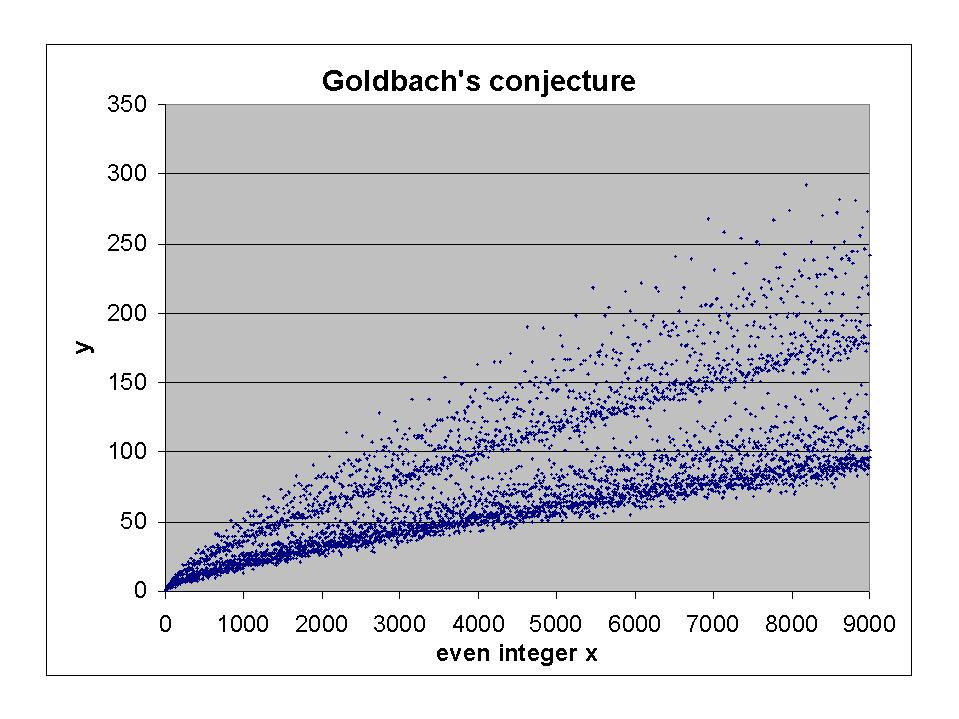
\includegraphics[width=10cm]{\imagePath/goldbach}
\caption{\label{goldbach}Eine Abbildung mit einer Bitmap aus dem Verzeichnis \lstinline$imagePath$}
\end{figure}
Neben Abbildungen, die mit EPS-Grafiken oder Bitmaps\randnotiz{Koordinaten-\\systeme} erstellt werden bietet \LaTeX{} die M�glichkeit mit
Vektorgrafik-Funktionen selbst Abbildungen zu zeichnen.

Seit September 2018 wird das \LaTeX{}-Paket
\lstinline$xpicture$ eingesetzt. Details findet man in der Dokumentation dieses Pakets
und in \cite{brill_18}. Der Dokumentation zu \datei{mbPDF.sty} sind auch die Abbildungen
\ref{floats:grid} und \ref{floats:polargrid} entnommen.

\begin{figure}[ht]
\definecolor{myblue}{cmyk}{1,1,0,0.5}
\renewcommand{\gridcolor}{myblue}
\renewcommand{\secundarygridcolor}{cyan}
\setlength{\gridthickness}{0.5pt}
\setlength{\secundarygridthickness}{0.1pt}
\renewcommand{\xunitdivisions}{3}
\renewcommand{\yunitdivisions}{3}
\renewcommand{\axeslabelsize}{\footnotesize}
\begin{center}
\setlength{\unitlength}{1cm}
\begin{Picture}(-3.5,-2.5)(3.5,2.5)
\cartesiangrid(-3.4,-2.4)(3.4,2.4)
\end{Picture}
\caption{\label{floats:grid}Ein kartesisches Koordinatensystem mit Gitterlinien (\lstinline$xpicture$)}
\end{center}
\end{figure}

\begin{figure}[ht]
\renewcommand{\runitdivisions}{2}
\setlength{\unitlength}{0.75cm}
\renewcommand{\gridcolor}{magenta}
\begin{center}
\begin{Picture}(-4,-4)(4,4)
\polargrid{3.5}{12}
\end{Picture}
\end{center}
\caption{\label{floats:polargrid}Ein Polarkoordinatensystem mit Koordinatenlinien (\lstinline$xpicture$)}
\end{figure}

Abbildung \ref{floats:grid} wurde mit dem folgenden Quelltext erzeugt:
\begin{lstlisting}{}
\definecolor{myblue}{cmyk}{1,1,0,0.5}
\renewcommand{\gridcolor}{myblue}
\renewcommand{\secundarygridcolor}{cyan}
\setlength{\gridthickness}{0.5pt}
\setlength{\secundarygridthickness}{0.1pt}
\renewcommand{\xunitdivisions}{3}
\renewcommand{\yunitdivisions}{3}
\renewcommand{\axeslabelsize}{\footnotesize}
\begin{center}
\setlength{\unitlength}{1cm}
\begin{Picture}(-3.5,-2.5)(3.5,2.5)
\cartesiangrid(-3.4,-2.4)(3.4,2.4)
\end{Picture}
\end{center}
\end{lstlisting}
Die Abbildung \ref{floats:polargrid} erh�lt man mit den folgenden Zeilen:
\begin{lstlisting}{}
\renewcommand{\runitdivisions}{2}
\setlength{\unitlength}{0.75cm}
\renewcommand{\gridcolor}{magenta}
\begin{center}
\begin{Picture}(-4,-4)(4,4)
\polargrid{3.5}{12}
\end{Picture}
\end{center}
\end{lstlisting}
Das Package \emph{xpicture} setzt \emph{calculator} und \emph{curves}
voraus. Insbesondere das Package \emph{calculator} bietet die M�glichkeit,
mathematische Konstanten und spezielle Funktionen abzurufen und mit Hilfe
von Variablen eigene Berechnungen und Funktionen zu definieren.
Die Abbildungen \ref{parameter7:zykloide} bis \ref{parameter7:trocho4}
sind mit dem folgenden Source-Code erzeugt worden:

\begin{lstlisting}{}
\begin{figure}[ht]
\COPY{2.0}{\radius}
\SUBTRACTfunction\IDENTITYfunction\SINfunction{\bracketOne}
\SCALEfunction{\radius}\bracketOne{\xfunction}
\SUBTRACTfunction\ONEfunction\COSfunction{\bracketTwo}
\SCALEfunction\radius\bracketTwo{\yfunction}
\PARAMETRICfunction{\xfunction}{\yfunction}{\myparfunction}
\centering
\setlength{\unitlength}{0.175cm}
\begin{Picture}(-36,-0.5)(31,6.5)
\pictcolor{orange}
\linethickness{1pt}
\PlotParametricFunction[48]{\myparfunction}{-16}{15}
\pictcolor{black}
\linethickness{0.5pt}
\xtrivVECTOR(-36.0, 0.0)(31.0, 0.0)
\end{Picture}
\caption{\label{parameter7:zykloide}Eine Zykloide 
mit $r=2$}

\vspace*{0.2cm}
\COPY{1.5}{\distance}
\SCALEfunction\radius\IDENTITYfunction{\Xone}
\SCALEfunction\distance\SINfunction{\Xtwo}
\SUBTRACTfunction\Xone\Xtwo{\xfunction}
\CONSTANTfunction{\radius}{\Yone}
\SCALEfunction\distance\COSfunction{\Ytwo}
\SUBTRACTfunction\Yone\Ytwo{\yfunction}
\PARAMETRICfunction{\xfunction}{\yfunction}{\myparfunction}
\begin{Picture}(-36,-0.5)(31,6.5)
\pictcolor{orange}
\linethickness{1pt}
\PlotParametricFunction[36]{\myparfunction}{-16}{15}
\pictcolor{black}
\linethickness{0.5pt}
\xtrivVECTOR(-36.0, 0.0)(31.0, 0.0)
\end{Picture}
\caption{\label{parameter7:trocho1}Eine Trochoide
 mit $r=2$ und $d=1{,}5$}

\vspace*{0.2cm}
\COPY{0.5}{\distance}
\begin{Picture}(-36,-0.5)(31,6.5)
\pictcolor{orange}
\linethickness{1pt}
\PlotParametricFunction[48]{\myparfunction}{-16}{15}
\pictcolor{black}
\linethickness{0.5pt}
\xtrivVECTOR(-36.0, 0.0)(31.0, 0.0)
\end{Picture}
\caption{\label{parameter7:trocho2}Eine Trochoide 
mit $r=2$ und $d=0{,}5$}

\vspace*{0.2cm}
\COPY{2.5}{\distance}
\begin{Picture}(-36,-1.5)(31,6.5)
\pictcolor{orange}
\linethickness{1pt}
\PlotParametricFunction[48]{\myparfunction}{-16}{15}
\pictcolor{black}
\linethickness{0.5pt}
\xtrivVECTOR(-36.0, 0.0)(31.0, 0.0)
\end{Picture}
\caption{\label{parameter7:trocho3}Eine Trochoide mit 
$r=2$ und $d=2{,}5$}

\vspace*{0.2cm}
\COPY{3.5}{\distance}
\begin{Picture}(-36,-1.5)(31,6.5)
\pictcolor{orange}
\linethickness{1pt}
\PlotParametricFunction[48]{\myparfunction}{-16}{15}
\pictcolor{black}
\linethickness{0.5pt}
\xtrivVECTOR(-36.0, 0.0)(31.0, 0.0)
\end{Picture}
\caption{\label{parameter7:trocho4}Eine Trochoide mit 
$r=2$ und $d=3{,}5$}
\end{figure}
\end{lstlisting}

\begin{figure}[ht]
\COPY{2.0}{\radius}
\SUBTRACTfunction\IDENTITYfunction\SINfunction{\bracketOne}
\SCALEfunction{\radius}\bracketOne{\xfunction}
\SUBTRACTfunction\ONEfunction\COSfunction{\bracketTwo}
\SCALEfunction\radius\bracketTwo{\yfunction}
\PARAMETRICfunction{\xfunction}{\yfunction}{\myparfunction}
\centering
\setlength{\unitlength}{0.175cm}
\begin{Picture}(-36,-0.5)(31,6.5)
\pictcolor{orange}
\linethickness{1pt}
\PlotParametricFunction[48]{\myparfunction}{-16}{15}
\pictcolor{black}
\linethickness{0.5pt}
\xtrivVECTOR(-36.0, 0.0)(31.0, 0.0)
\end{Picture}
\caption{\label{parameter7:zykloide}Eine Zykloide mit $r=2$}

\vspace*{0.2cm}
\COPY{1.5}{\distance}
\SCALEfunction\radius\IDENTITYfunction{\Xone}
\SCALEfunction\distance\SINfunction{\Xtwo}
\SUBTRACTfunction\Xone\Xtwo{\xfunction}
\CONSTANTfunction{\radius}{\Yone}
\SCALEfunction\distance\COSfunction{\Ytwo}
\SUBTRACTfunction\Yone\Ytwo{\yfunction}
\PARAMETRICfunction{\xfunction}{\yfunction}{\myparfunction}
\begin{Picture}(-36,-0.5)(31,6.5)
\pictcolor{orange}
\linethickness{1pt}
\PlotParametricFunction[36]{\myparfunction}{-16}{15}
\pictcolor{black}
\linethickness{0.5pt}
\xtrivVECTOR(-36.0, 0.0)(31.0, 0.0)
\end{Picture}
\caption{\label{parameter7:trocho1}Eine Trochoide mit $r=2$ und $d=1{,}5$}

\vspace*{0.2cm}
\COPY{0.5}{\distance}
\begin{Picture}(-36,-0.5)(31,6.5)
\pictcolor{orange}
\linethickness{1pt}
\PlotParametricFunction[48]{\myparfunction}{-16}{15}
\pictcolor{black}
\linethickness{0.5pt}
\xtrivVECTOR(-36.0, 0.0)(31.0, 0.0)
\end{Picture}
\caption{\label{parameter7:trocho2}Eine Trochoide mit $r=2$ und $d=0{,}5$}

\vspace*{0.2cm}
\COPY{2.5}{\distance}
\begin{Picture}(-36,-1.5)(31,6.5)
\pictcolor{orange}
\linethickness{1pt}
\PlotParametricFunction[48]{\myparfunction}{-16}{15}
\pictcolor{black}
\linethickness{0.5pt}
\xtrivVECTOR(-36.0, 0.0)(31.0, 0.0)
\end{Picture}
\caption{\label{parameter7:trocho3}Eine Trochoide mit $r=2$ und $d=2{,}5$}

\vspace*{0.2cm}
\COPY{3.5}{\distance}
\begin{Picture}(-36,-1.5)(31,6.5)
\pictcolor{orange}
\linethickness{1pt}
\PlotParametricFunction[48]{\myparfunction}{-16}{15}
\pictcolor{black}
\linethickness{0.5pt}
\xtrivVECTOR(-36.0, 0.0)(31.0, 0.0)
\end{Picture}
\caption{\label{parameter7:trocho4}Eine Trochoide mit $r=2$ und $d=3{,}5$}
\end{figure}
%
\section{Tabellen}
\begriff{Tabellen} werden mit \datei{table} eingef�gt und haben immer eine Beschriftung, um
im Text darauf Bezug zu nehmen. Die Beschriftung wird als Tabellen-�berschrift
eingef�gt, also oberhalb der Tabelle. Das stammt aus den Projekten mit dem Hanser-Verlag
und wurde seitdem beibehalten. Bei den B�chern wurde die Quelle f�r jede Tabelle
sogar in separate Dateien ausgelagert und in einem Verzeichnis \datei{tables}
zusammengefasst. Dies ist sinnvoll wenn Tabellen sowohl in einem Text als auch
in Folien, die man mit dem \begriff{Beamer}-Paket erstellt, verwendet. So ist sicher gestellt,
dass die Tabelle nur an einer Stelle steht und dass Korrekturen so immer f�r alle Dokumente
wirken, in denen die Tabelle verwendet wird.

\begin{table}[ht]
\centering
\caption{\label{tabelle}Ein Beispiel f�r eine Tabelle}
\begin{tabular}{ll}\hline
\textbf{Erste Spalte}&\textbf{Zweite Spalte}\\\hline
$1$&Eins\\
$2$&Zwei\\\hline
\end{tabular}
\end{table}
Die Tabelle \ref{tabelle}
wurde mit dem folgenden Quelltext eingef�gt:

\begin{lstlisting}{}
\begin{table}[ht]
\centering
\begin{tabular}{ll}\hline
\textbf{Erste Spalte}&\textbf{Zweite Spalte}\\\hline
Erste Spalte&Zweite Spalte\\\hline
$1$&Eins\\
$2$&Zwei\\\hline
\end{tabular}
\end{table}
\end{lstlisting}
Eintr�ge in den Spalten sind meist linksb�ndig. Das muss man nicht beibehalten, aber
die Ausrichtung von Eintr�gen sollte immer konsistent sein.

%
%
\chapter{Verzeichnisse und Index}
\section{Literaturverzeichnis}
Das \begriff{Literaturverzeichnis} wird mit Hilfe von \bibtex{} aufgebaut. \bibtex{} ist relativ alt und unhandlich, das macht sich h�ufig bemerkbar. Es ist geplant auf
\emph{BibLaTeX} umzusteigen.

Die einzelnen Eingabe-Dateien f�r die Quellen werden mit Hilfe von \jabref{}, einer
\java{}-Anwendung\randnotiz{JabRef}\index{JabRef}, verwaltet (\cite{jabref}). Vorteil dieser Anwendung ist, dass man in den Dateien suchen kann
und die Eintr�ge als Formular-Eintr�ge bearbeitet werden k�nnen. Das Literaturverzeichnis,
das wir auf Seite \pageref{literatur} finden wurde so in das Dokument eingef�gt:

\begin{lstlisting}{}
\cleardoublepage
\phantomsection
\addcontentsline{toc}{chapter}{Literaturverzeichnis}
\chaptermark{Literaturverzeichnis}
\sectionmark{Literatur}\label{literatur}
\bibliography{../../../BibTex/latex}
\end{lstlisting}
Interessant ist die Funktion \lstinline$phantomsection$, die daf�r sorgt, dass das Literaturverzeichnis
richtig behandelt wird und die Verweise in der Inhaltsangabe bei der \pdf{}-Anzeige auch
korrekt auf den Anfang des Literaturverzeichnisses verweisen.
%
\section{Index}
Der \begriff{Index} wird mit dem Paket \lstinline$imakeidx$ erzeugt. Hier ist wichtig, dass die deutschen Umlaute korrekt
dargestellt werden. Dies gelingt durch die Option \lstinline$-g$ f�r die Funktion \lstinline$makeindex$, die
w�hrend der Erstellung des \pdf{}-Dokuments aufgerufen wird. Damit diese Option korrekt arbeitet und
deutsche Umlaute wie gewohnt im Editor eingegeben werden k�nnen m�ssen die Quotes umgestellt werden. Dazu gibt
es die Datei \datei{german.ist}, die sinnvoller Weise in \datei{texmf-local/makeindex/german} gespeichert ist:\index{Index!deutsche Umlauge}
\begin{lstlisting}{}
% Voraussetzung: makeindex mit Option -g aufrufen!
quote '>'    % > ersetzt "
%
delim_0 "\\hspace{2ex} "
delim_1 "\\hspace{2ex} "
delim_2 "\\hspace{2ex} "
\end{lstlisting}
F�r den Index ist eingestellt, dass ein Eintrag im Inhaltsverzeichnis erstellt wird und dass der Index, der mit \lstinline$printindex$
ausgegeben wird, zweispaltig ist. In diesem Dokument wurde der Index so eingef�gt:
\begin{lstlisting}{}
% Index
\clearevenpage
\phantomsection
\small
\printindex
\normalsize
\end{lstlisting}

%
%
% Literatur
%
\cleardoublepage
\phantomsection
\addcontentsline{toc}{chapter}{Literaturverzeichnis}
\chaptermark{Literaturverzeichnis}
\sectionmark{Literatur}\label{literatur}
\bibliography{latex}
%
% Anhang
%
\appendix
%
\chapter*{L�sungshinweise}\label{solhinweise}
Hier finden sich die beiden Beispiele f�r die L�sungshinweise.

\hinweis{stat17}
\hinweis{stat22}
%
% Index
\clearevenpage
\phantomsection
\small
\printindex
\normalsize
\end{document}
